\documentclass[conference]{IEEEtran}
\usepackage{cite,amsmath,amssymb,graphicx,booktabs,url,xcolor,array}
\newcolumntype{L}[1]{>{\raggedright\arraybackslash}p{#1}}
\usepackage{pgfplots}
\pgfplotsset{compat=1.17}
\newcommand{\need}[1]{\textcolor{red}{[NEED: #1]}}
\newcommand{\bcm}{\textsc{BCM}}
\newcommand{\RQ}[2]{\textbf{RQ#1 (#2)}}

\begin{document}

\title{What Does the Behavioral Consistency Metric Measure? A Construct-Validity Study of Attribution-Based Consistency for Software Engineering Agents}

\author{\IEEEauthorblockN{[Author 1]}
\IEEEauthorblockA{[Affiliation]\\
\relax [email]}
\and
\IEEEauthorblockN{[Author 2]}
\IEEEauthorblockA{[Affiliation]\\
\relax [email]}
\and
\IEEEauthorblockN{[Author 3]}
\IEEEauthorblockA{[Affiliation]\\
\relax [email]}
\and
\IEEEauthorblockN{[Author 4]}
\IEEEauthorblockA{[Affiliation]\\
\relax [email]}}

\maketitle

\begin{abstract}
Software engineering agents are ranked by how many issues they resolve, and the Behavioral Consistency Metric (\bcm) has been proposed to add how consistently they behave: it is the mean pairwise cosine similarity of SHAP attributions from a classifier that predicts success from trajectory features. We test whether \bcm{} measures agent behaviour or the parser, predictor and tasks behind it. We audit and re-implement the released pipeline on 9{,}191 trajectories, recompute \bcm{} on 9{,}139 public SWE-bench Pro trajectories from one scaffold, and run a controlled experiment with five open-weight agents (4{,}645 attempts on 111 SWE-bench Verified tasks) that adds repeated runs and execution-validated task variants, reviewed by two human raters. The published values are reproduced only by a predictor that selected its size on the fold it scored, and the released parser reads 2{,}513 of 4{,}000 trajectories as empty. Changing only the parser moves GPT-5 from first (\bcm{} 0.554) to last place (0.041). \bcm{} is no higher than its value under permuted success labels for all five archival models and for four of five controlled agents, although the predictor separates outcomes within every agent (AUC 0.76--0.97). The agent that solves 1.3\% of its attempts receives the highest score (0.259). Attribution similarity between two runs of the same task does follow whether they pass the same tests ($r=0.25$), but such pairs are 0.7\% of the pairs \bcm{} averages. \bcm{} therefore reflects how a pooled predictor's attributions concentrate, not consistent behaviour; consistency should be measured on repeated runs of the same task.
\end{abstract}

\begin{IEEEkeywords}
software engineering agents, evaluation metrics, construct validity, explainability, SHAP, SWE-bench
\end{IEEEkeywords}

%% ==================================================================
\section{Introduction}
\label{sec:intro}
Consider five open-weight coding agents run under one scaffold, each attempting the same set of GitHub issues three to five times. One of them, Qwen2.5-Coder-7B, resolves 1.3\% of its attempts and is the least repeatable of the five: its runs on the same issue share fewer actions than those of any other agent. A consistency metric should rank it low. The Behavioral Consistency Metric~\cite{raichura2026bcm} ranks it first. This paper explains why, and what that says about the metric.

Benchmarks such as SWE-bench~\cite{jimenez2024swebench} and SWE-bench Verified~\cite{openai2024verified} score an agent by the share of issues whose hidden tests pass after its patch. Teams that adopt an agent for code review, issue triage or automated repair need more than this number. Two agents with the same solve rate can differ in how predictably they behave, and an agent whose behaviour changes from run to run is harder to review, debug and budget for. Leaderboards and tool vendors therefore look for process-level measures that can be computed from the trajectories agents already record.

Banerjee and Raichura proposed \bcm{} as such a measure~\cite{raichura2026bcm}. \bcm{} turns each trajectory into a vector of trace features, such as step counts, action types and error counts; trains a gradient-boosted classifier~\cite{ke2017lightgbm} to predict whether the trajectory resolved its task; computes a SHAP attribution vector~\cite{lundberg2017shap,lundberg2020treeshap} for each trajectory; and reports, per agent, the mean pairwise cosine similarity of those vectors. The authors read a high value as stable, success-relevant decision patterns, and report that proprietary models score higher than open-weight ones.

That reading assumes that the attributions describe the agent. They describe a predictor that is trained on the trajectories of several agents together, on features produced by a log parser, over trajectories from different tasks. Each of these steps can make attribution vectors similar without any similarity in what the agents did. Whether a score measures the property it is named after is a question of \emph{construct validity}~\cite{cronbach1955construct,messick1995validity}. To our knowledge, \bcm{} has not been compared with a value that carries no outcome information, nor with an independent measure of whether two runs behaved alike.

We test the construct validity of \bcm{} by separating three sources of variation that any such score combines: the \emph{measurement} (parser, features, predictor, explainer), the \emph{task} (which issue and repository a trajectory comes from) and the \emph{agent} (what it actually did). Four studies each remove an explanation that the previous one leaves open. A replication and an independent re-implementation audit the released pipeline. An archival study of public SWE-bench Pro trajectories~\cite{deng2025swebenchpro} holds the scaffold fixed and varies only the measurement. A controlled experiment adds what archives lack: repeated runs on the same task, and task variants whose correct behaviour is fixed by executable tests rather than by \bcm. Two human raters checked the model-generated variants and the automatic labels.

The four studies agree. \bcm{} values are reached without outcome information, a parser change alone reverses a ranking, and a predictor trained on one agent at a time gives \bcm{} values near zero. The controlled experiment shows why the failing agent ranks first: \bcm{} averages over pairs of trajectories from different tasks, which are more than 99\% of all pairs, so it measures where an agent's trajectories sit in the pooled feature space. The signal that attributions do carry is in pairs of runs on the same task, and \bcm{} averages it away. The paper makes four contributions:
\begin{enumerate}
\item An audit that traces the published \bcm{} values to three pipeline choices: a validation-leaky model selection, a parser that loses the steps of 2{,}513 trajectories, and the pooling of agents in one predictor (RQ1).
\item Evidence from released, archival and controlled data that \bcm{} is not above a label-permutation null for most agents and does not follow repeatability (RQ2).
\item Evidence that attribution similarity on same-task pairs tracks whether two runs pass the same tests, which locates the usable signal that \bcm{} discards (RQ3), together with invariance and adaptation tests on execution-validated task variants (RQ4, RQ5).
\item A reusable validation protocol for trajectory-level agent metrics, with a replication package containing all code, manifests, model revisions and human labels (Section~\ref{sec:replication}).
\end{enumerate}

%% ==================================================================
\section{Background: the Behavioral Consistency Metric}
\label{sec:background}
A software engineering agent receives an issue and a repository. It alternates between calls to a language model and actions in a shell, such as searching files, editing them and running tests, until it submits a patch. We call the recorded sequence of actions and observations a \emph{trajectory}. An attempt \emph{resolves} its task if the issue's target tests (FAIL\_TO\_PASS) pass after the patch and the previously passing tests (PASS\_TO\_PASS) still pass~\cite{jimenez2024swebench}.

For an agent $s$ with trajectories $i=1,\dots,n_s$, let $x_i$ be the trace-feature vector and $y_i\in\{0,1\}$ the outcome. A classifier $f$ is trained in cross-validation to predict $y$ from $x$; the original work uses LightGBM on the trajectories of all agents together. For each trajectory, scored by the model that did not see it, the SHAP vector $\phi_i\in\mathbb{R}^d$ gives each feature's contribution to the predicted log-odds. Then
\[
\bcm(s)=\frac{2}{n_s(n_s-1)}\sum_{i<j}\frac{\phi_i\cdot\phi_j}{\lVert\phi_i\rVert\,\lVert\phi_j\rVert}.
\]
\bcm{} is 1 if all of an agent's attribution vectors point in the same direction, and near 0 if they point in unrelated directions.

The released pipeline offers a concrete case of a high value without consistent behaviour. Its parser returns zero steps for 2{,}513 of 4{,}000 SWE-smith trajectories (Section~\ref{sec:rq1}). Every trajectory with zero steps has the same feature vector, so within one cross-validation fold it receives the same attribution vector, and every pair of such trajectories has cosine 1. In the shipped results, empty rows contribute exactly five distinct attribution vectors per agent, one per fold, and excluding them lowers Claude-3.7's \bcm{} from 0.766 to 0.514.

The example is one of four ways in which \bcm{} can be high or low for reasons other than agent behaviour. \emph{Pooling}: because $f$ is trained on several agents, an agent whose trajectories differ from the others in one feature, such as length, receives attributions that all point along that feature. \emph{Attributions explain the predictor}: SHAP values describe the model, not the process that generated the data~\cite{kumar2020shapproblems}, and attribution methods can look plausible while being insensitive to the model or the labels~\cite{adebayo2018sanity}. \emph{Representation}: the features come from a parser, and parsers differ in which trajectories they extract steps from. \emph{Task structure}: \bcm{} compares trajectories from different tasks, so differences between tasks can dominate the similarity.

%% ==================================================================
\section{Study Design}
\label{sec:design}
\subsection{Research questions}
Each research question targets one of the alternative explanations above and states which answer would count against the intended reading of \bcm.

\RQ{1}{Measurement Dependence}. How much do \bcm{} values and rankings change with the parser, the representation, the predictor and the set of pooled agents? Large changes under choices that do not change the agent show that the value is partly a property of the measurement.

\RQ{2}{Outcome Dependence}. Does \bcm{} exceed its value when success labels are permuted within an agent, which removes any link between trajectory and outcome? A value at or below this null is not evidence of success-relevant behaviour.

\RQ{3}{Behavioural Agreement}. For two runs of the same agent on the same task, does attribution similarity follow independent, task-grounded evidence that the runs did similar things, beyond the similarity of their raw features?

\RQ{4}{Rewording Invariance}. Do behaviour and attributions stay the same when the issue text is reworded without changing the task?

\RQ{5}{Requirement Adaptation}. When the correct behaviour changes, do agents adapt, and can attributions tell an agent that adapted from one that kept the old behaviour?

\subsection{Study parts}
Table~\ref{tab:design} lists the five parts of the study. Parts 1 and 2 use the original data, so they cannot separate the agent from its data source. Part 3 holds the scaffold and benchmark fixed but has one attempt per task, so it cannot test repeatability. Part 4 adds repeated runs and controlled task variants, and Part 5 checks the inputs of Part 4 that a model generated or a program labelled.

\begin{table*}[t]
\centering
\caption{The five parts of the study, the data each uses, what each varies, and the research questions each answers.}
\label{tab:design}
\begin{tabular}{llll}
\toprule
Part & Data & Varied & RQ\\
\midrule
1 Replication & 9{,}191 released trajectories (SWE-smith, Nebius), 6 agents & pipeline stages & 1, 2\\
2 Re-implementation & same data, independent code & predictor, null & 1, 2\\
3 Archival & 9{,}139 SWE-bench Pro trajectories, 13 runs, one scaffold & parser, predictor, pooling & 1, 2\\
4 Controlled experiment & 4{,}645 attempts, 5 open-weight agents, 111 tasks & repeats, task variants & 2--5\\
5 Human review & 368 items, each rated by 2 raters & --- & checks Part 4\\
\bottomrule
\end{tabular}
\end{table*}

\textbf{Parts 1 and 2: replication and re-implementation.} We reran the authors' released pipeline on the 9{,}191 SWE-smith and Nebius trajectories it uses, regenerated the shipped attribution matrix, and examined the git history of the predictor configuration. We then tested each stage separately: parsing, features, predictor, explainer and aggregation. Part 2 re-implemented predictor, attribution and \bcm{} without importing the audited code; it reused only the feature tables after checking them against the shipped matrix. Controls were label permutations within agent, and within agent and repository (50 seeds each), a logistic-regression predictor, and a role-aware parser that counts one step per action the model proposed.

\textbf{Part 3: archival trajectories.} We used 9{,}139 public SWE-agent trajectories from 13 SWE-bench Pro runs~\cite{deng2025swebenchpro}. The primary cohort is five models (GPT-5, Claude Sonnet-4.5, Claude Haiku-4.5, GLM-4.5 and Gemini-2.5-Pro) under one 250-turn configuration, which we confirmed by comparing the run configurations, on the 715 tasks all five attempted. Outcomes follow the official rule applied to the archived test outputs. We computed \bcm{} under four representations (the authors' two loaders, the role-aware parser and a tool-semantic parser) and several predictor families, with task-grouped and leave-one-repository-out cross-validation.

\textbf{Part 4: controlled experiment.} We drew tasks from SWE-bench Verified with a seeded rule stratified by repository and difficulty, capping Django at 30\%. A task was replaced by the next one in its stratum only if it failed an executable check: the reference patch must resolve it and the empty patch must not. The set has 99 tasks from 11 repositories, plus 12 extension tasks used only for the changed-requirement condition. All five models ran under one scaffold, mini-SWE-agent 2.4.6 with its text-based action format~\cite{minisweagent}, with identical prompts, sampling (temperature 0.7, top-$p$ 0.8), a 50-step limit, a 32k-token context and a one-hour cap per attempt, served locally with vLLM~\cite{kwon2023vllm}. The four primary models are Qwen3-Coder-30B-A3B, Devstral-Small-2507, SWE-agent-LM-32B and Qwen2.5-Coder-32B; Qwen2.5-Coder-7B was included in advance as a control that rarely succeeds. A staging gate (at least three distinct tasks solved and format compliance of at least 0.90) excluded gpt-oss-120b (compliance 0.656). Llama-3.3-70B was planned, but its weights require an access approval we did not have, so no model larger than 32B is included. Each attempt ran in a fresh Apptainer sandbox built from the task's official SWE-bench image; every agent command starts in the task's conda environment, and before each attempt the harness checks that the interpreter belongs to that environment and that the repository imports from its working copy. The official grader uses the same environment.

Table~\ref{tab:variants} defines the five task variants. Every variant was validated by execution before use. C2 drafts were produced by local open-weight models (GLM-4-32B and gpt-oss-120b), because a purely mechanical version, which replaces a message literal that the fix adds and the tests check, is possible for only 1 of the 500 Verified tasks. A rejected draft could be revised using the measured failure, but the acceptance rules never changed and no draft was edited by hand. Of the 99 main tasks, 58 (59\%) received an accepted B2 and 33 (33\%) an accepted C2; C2 acceptance ranged from 11\% (matplotlib) to 67\% (xarray) by repository.

\begin{table}[t]
\centering
\caption{Task variants in Part 4. Each variant passed its acceptance check before any agent ran on it.}
\label{tab:variants}
\footnotesize
\setlength{\tabcolsep}{3pt}
\begin{tabular}{L{1.25cm}L{3.0cm}L{3.6cm}}
\toprule
Variant & Change to the task & Acceptance check\\
\midrule
A original & none & reference patch resolves, empty patch does not\\
B1 control & whitespace and a neutral framing sentence & code and identifiers unchanged\\
B2 reworded & prose rewritten by a model; code, identifiers, paths, numbers and quoted strings masked and restored & every masked item restored once, nothing protected added, prose sequence similarity $\le 0.6$\\
C1 already fixed & reference fix applied and committed; issue unchanged & correct decision is to check and change nothing\\
C2 changed requirement & appended maintainer update; matching edits to fix and hidden tests & under revised tests: unchanged repository fails, revised fix passes, original fix fails; update states every new tested literal\\
\bottomrule
\end{tabular}
\end{table}

Condition A ran on 111 tasks with five repeats for the primary models (99 tasks and three repeats for the 7B control), B2 on 58 tasks and C2 on 45 tasks with four repeats, and B1 and C1 on a 20-task subset with three repeats: 4{,}645 attempts in total, all completed and graded. Attempts interrupted by the infrastructure were restarted from scratch with the same seed. Most primary-model attempts ran on NVIDIA RTX PRO 6000 GPUs (two cards for the 32B models) and the 7B control on an L40S; because the RTX nodes became unavailable during the experiment, 489 attempts (317 of Devstral, 172 of SWE-agent-LM) ran on H200 GPUs.

\subsection{Measures}
We keep three constructs apart: \emph{behavioural consistency} (whether two runs on the same task did the same thing), \emph{task appropriateness} (editing only when needed, without regressions) and \emph{final correctness} (the tests pass). The two co-primary measures of behavioural consistency are task-grounded: agreement on the per-test status of the FAIL\_TO\_PASS tests (\emph{test agreement}), and Jaccard similarity of the normalised changed source lines, defined when both runs edited source (\emph{changed-line similarity}). Agreement on whether to edit and the Jaccard similarity of edited functions are secondary. Similarity of the two runs' action-category sequences (\emph{sequence similarity}) comes from the same trajectory as the \bcm{} features, so we report it only as a reference, never as validation. For C1 we classify each attempt as a verified no-op, a correct decision submitted as text, inaction, a harmless edit, or a harmful edit (a previously passing test fails); for C2, as adapted (revised tests pass), persisted (original tests pass, revised tests fail) or failed. Because agents sometimes state the right decision but submit a sentence rather than a diff, we also grade the final repository state.

\subsection{Attribution pipeline and analysis}
We used the released LightGBM configuration with tree-path TreeSHAP as the primary predictor and explainer, with a standardised logistic regression and a tool-semantic representation as alternatives; task-grouped five-fold cross-validation over 10 seeds; and 50-seed nulls with labels permuted within model, and within model and repository. TreeSHAP additivity was asserted to $10^{-6}$ on every fold (largest error $2.2\times10^{-14}$). We did not use the shap package's interventional explainer: in Part 2 we found that it silently subsamples any background dataset larger than 100 rows, so its values refer to a random subset of the background supplied; exact interventional values over the full background leave every conclusion unchanged.

The analysis plan, including hypotheses, measures, margins and exclusions, was fixed before the controlled attempts were run and is included in the replication package. Uncertainty uses task-cluster bootstrap intervals (2{,}000 resamples), with repository-cluster resampling as a sensitivity analysis. The 7B control is reported separately and excluded from pooled estimates, because an agent that always fails can be consistent. For RQ3, H1 states that the within-task correlation between attribution cosine and each co-primary measure is positive (Bonferroni-adjusted lower bound above 0) and calls it substantive if the lower bound exceeds 0.1; we also report it after partialling out the similarity of the two runs' raw feature vectors. For RQ4, H2 states that the difference between A-vs-A and A-vs-B2 similarity lies within $\pm0.05$ for four co-primary measures (two one-sided tests~\cite{schuirmann1987tost,lakens2018equivalence}, Bonferroni-adjusted); the solve-rate difference is estimated only, because 58 tasks give a power of 0.26 for its equivalence test. For RQ5, H3 estimates per-model adaptation and persistence rates, and H4 tests the AUC with which the attribution-based margin separates adapted from persisted attempts; with fewer than 50 persisted attempts, H4 is reported as inconclusive.

\subsection{Human review}
\label{sec:humandesign}
A program or a model produced several inputs of Part 4: the B2 rewrites, the C2 updates, fixes and tests, and the C1 classes. Two raters, both PhD students in our research lab who remain anonymous, reviewed them independently, together with the parser outputs of Parts 1 and 3 and an automatic localisation measure of Part 3. The raters received a package without any automatic or AI verdict, without outcome labels, and with model names replaced by codes; both labelled every row without discussing items, and neither used AI tools. The items were 33 B2 rewrites and 33 C2 variants (three staging tasks plus a seeded sample of 30 that covers 30 of the 58 B2 and 30 of the 45 C2 tasks analysed); 54 C1 attempts from the pilot, stratified by class and model, which validate the automatic C1 classes; 200 submitted patches from Part 3 (40 tasks, five models), judged for whether they edit the place the reference fix edits; and 24 parsed steps each from Parts 1 and 3. We report percentage agreement, Cohen's $\kappa$~\cite{cohen1960kappa} and Gwet's AC1~\cite{gwet2008ac1}, which is less affected than $\kappa$ when almost all labels fall into one category~\cite{feinstein1990paradox}. We do not exclude tasks on the question ``does the rewrite read naturally'', because the raters agreed on it no better than chance.

%% ==================================================================
\section{Results}
\label{sec:results}
Each research question is answered in one subsection. A validity check of the task variants precedes RQ4 and RQ5, which depend on them.

\subsection{RQ1: Measurement Dependence}
\label{sec:rq1}
\textbf{Leaky model selection.} The released script does not regenerate the shipped attribution matrix: it gives a pooled AUC of 0.728, not the shipped 0.690. An earlier predictor configuration from the authors' git history reproduces the shipped out-of-fold probabilities and SHAP matrix exactly (largest difference 0.0). This configuration selects the number of trees by early stopping on the fold it then scores. The selected sizes per fold are 173, 225, 66, 82 and 4 trees, so one fold's attributions come from a four-tree model chosen on the rows it explains.

\textbf{Parsing.} The authors' loader returns zero steps for 2{,}513 of 4{,}000 SWE-smith trajectories, and all 2{,}513 contain real tool calls. The loader also treats the two data sources differently: for SWE-smith it keeps the model's thought text as the step, and only 3.6\% of these steps contain the executed command; for Nebius it counts every message, including system prompts and tool output. Both human raters judged all 24 sampled role-aware steps to be real agent actions.

\textbf{Parser and pooling on one scaffold.} Part 3 removes the differences of source and scaffold that Parts 1 and 2 cannot separate from the agent. GPT-5 hides its reasoning, so 58\% of its trajectories parse to zero steps under the authors' loader. It ranks first under that loader (\bcm{} 0.554, 95\% CI [0.538, 0.570]) and last under role-aware parsing (0.041 [0.031, 0.052]). When the predictor is trained on one model's trajectories at a time, \bcm{} is 0.001 to 0.019 for every model, although these predictors are informative (within-model AUC 0.61 to 0.77). \bcm{} grows with the number of models pooled: Kimi-K2 has \bcm{} 0.006 alone and 0.505 with two other models, because one length feature places all its trajectories on one side of the pooled predictor.

\textbf{Answer to RQ1.} \bcm{} values and rankings depend on the measurement: a leaky model selection and a parser defect produced the published values, a parser change reverses a ranking on fixed data, and pooling creates the magnitude that per-model predictors do not show.

\subsection{RQ2: Outcome Dependence}
\label{sec:rq2}
In Part 1, with labels permuted within agent, the paper's own predictor gives the two Claude agents a median \bcm{} of 0.955, above their published values of 0.83 and 0.77. Under role-aware parsing, real \bcm{} is below the mean of its within-agent null in 17 of 18 agent-by-predictor cells, and the published gap between proprietary and Llama agents shrinks about fourfold, disappears with a logistic predictor, and largely survives permuting labels within repository. In Part 3, on the matched cohort of five models and 715 tasks, real \bcm{} (0.04 to 0.13) lies within the 5--95\% band of its within-model null for all five models, with LightGBM and with logistic regression; under the tool-semantic representation, three models modestly exceed their nulls.

Figure~\ref{fig:bcm} and Table~\ref{tab:permodel} give the Part 4 result. For four of five models, real \bcm{} is not above the within-model null, although the predictor separates success from failure within every model (AUC 0.76 to 0.97; pooled 0.86 against a null of 0.59). For Qwen3 and the 7B control it lies within the central 95\% of the null; for Devstral and SWE-agent-LM it lies below, so the real labels make attributions less aligned than random labels do. Only Qwen2.5-Coder-32B exceeds both the within-model null and the null that also preserves repository-level success rates ($p=0.02$ for both). With a logistic predictor or the tool-semantic representation, real \bcm{} is again within or below its null for at least four of five models.

\begin{figure}[t]
\centering
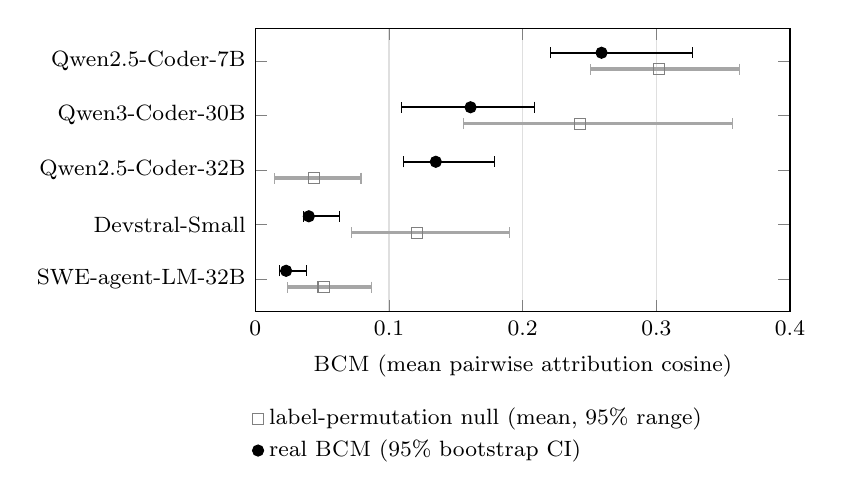
\begin{tikzpicture}
\begin{axis}[
  scale only axis, width=0.56\columnwidth, height=3.6cm,
  xmin=0, xmax=0.4, ymin=0.4, ymax=5.6,
  ytick={1,2,3,4,5},
  yticklabels={SWE-agent-LM-32B, Devstral-Small, Qwen2.5-Coder-32B, Qwen3-Coder-30B, Qwen2.5-Coder-7B},
  yticklabel style={font=\footnotesize},
  xticklabel style={font=\footnotesize, /pgf/number format/fixed},
  xlabel={\footnotesize \bcm{} (mean pairwise attribution cosine)},
  xmajorgrids, grid style={gray!25},
  legend style={font=\footnotesize, at={(0.42,-0.30)}, anchor=north, draw=none},
  legend cell align=left,
]
\addplot[only marks, mark=square, mark size=2pt, gray, mark options={fill=white}, error bars/.cd, x dir=both, x explicit, error bar style={line width=1.2pt, gray!70}]
coordinates {
 (0.051,0.85) += (0.036,0) -= (0.027,0)
 (0.121,1.85) += (0.069,0) -= (0.049,0)
 (0.044,2.85) += (0.035,0) -= (0.030,0)
 (0.243,3.85) += (0.114,0) -= (0.087,0)
 (0.302,4.85) += (0.060,0) -= (0.051,0)
};
\addlegendentry{label-permutation null (mean, 95\% range)}
\addplot[only marks, mark=*, mark size=2pt, black, mark options={fill=black}, error bars/.cd, x dir=both, x explicit, error bar style={line width=0.8pt, black}]
coordinates {
 (0.023,1.15) += (0.015,0) -= (0.005,0)
 (0.040,2.15) += (0.023,0) -= (0.004,0)
 (0.135,3.15) += (0.044,0) -= (0.024,0)
 (0.161,4.15) += (0.048,0) -= (0.052,0)
 (0.259,5.15) += (0.068,0) -= (0.038,0)
};
\addlegendentry{real \bcm{} (95\% bootstrap CI)}
\end{axis}
\end{tikzpicture}
\caption{\bcm{} per model in the controlled experiment (condition A) against its within-model label-permutation null. Only Qwen2.5-Coder-32B lies above its null; Devstral and SWE-agent-LM lie below. The model with the highest \bcm{}, Qwen2.5-Coder-7B, solves 1.3\% of its attempts.}
\label{fig:bcm}
\end{figure}

\textbf{Answer to RQ2.} \bcm{} does not depend on the outcome in the way its reading assumes: across released, archival and controlled data it is no higher than its label-permutation null for most agents, and the failing control receives the highest score.

\subsection{RQ3: Behavioural Agreement}
\label{sec:rq3}
\bcm{} averages over all pairs of an agent's trajectories, and pairs from the same task are 0.7\% of them, so \bcm{} is almost equal to the mean cosine of pairs from different tasks. For Qwen3, \bcm{} is 0.155, the different-task mean 0.153 and the same-task mean 0.418. Table~\ref{tab:permodel} shows that the \bcm{} ranking does not follow repeatability: ordered by changed-line similarity between repeats, the models rank Qwen3, SWE-agent-LM, Qwen2.5-32B, Devstral and the 7B control. Test agreement is highest for the 7B control (0.98) because almost all of its runs fail the same tests, which is why repeat-based measures must be read with the solve rate.

\begin{table}[t]
\centering
\caption{Per-model results of the controlled experiment (condition A). Solve: share of resolved attempts. \bcm{}, its two-sided permutation $p$-value against the within-model null, and the within-model predictor AUC. Repeatability: mean similarity of repeat pairs on the same task.}
\label{tab:permodel}
\footnotesize
\setlength{\tabcolsep}{2.4pt}
\begin{tabular}{lrrrrrrr}
\toprule
 & & \multicolumn{3}{c}{\bcm} & \multicolumn{3}{c}{Repeatability}\\
\cmidrule(lr){3-5}\cmidrule(lr){6-8}
Model & Solve & value & $p$ & AUC & tests & lines & seq.\\
\midrule
Qwen2.5-Coder-7B & 0.013 & 0.259 & 0.22 & 0.97 & 0.980 & 0.109 & 0.237\\
Qwen3-Coder-30B & 0.261 & 0.161 & 0.18 & 0.76 & 0.773 & 0.269 & 0.460\\
Qwen2.5-Coder-32B & 0.115 & 0.135 & 0.02 & 0.84 & 0.868 & 0.168 & 0.379\\
Devstral-Small & 0.270 & 0.040 & 0.04 & 0.89 & 0.804 & 0.165 & 0.499\\
SWE-agent-LM-32B & 0.159 & 0.023 & 0.10 & 0.88 & 0.815 & 0.173 & 0.379\\
\bottomrule
\end{tabular}
\end{table}

Within a task, attribution cosine correlates with test agreement ($r_w=0.245$, 97.5\% CI [0.182, 0.310]) and with changed-line similarity (0.132 [0.097, 0.175]). H1 is supported for both; for test agreement the lower bound also exceeds the pre-specified substantive value of 0.1, for changed lines it does not. Attribution cosine follows the trace-derived sequence similarity more closely (0.415 [0.368, 0.461]). After partialling out the similarity of the two runs' raw feature vectors, the test-agreement correlation stays at 0.208 [0.146, 0.268], while the changed-line correlation falls to 0.060 [0.018, 0.099]. These decisions hold under repository-cluster resampling and with logistic or tool-semantic attributions, and the test-agreement intervals exclude zero for each of the four primary models.

\textbf{Answer to RQ3.} Attribution similarity on same-task pairs carries information about whether two runs reach the same test outcomes that the raw features do not, and little about whether they change the same lines. \bcm{} discards this signal because it averages over different-task pairs.

\subsection{Validity of the task variants and labels}
\label{sec:human}
Table~\ref{tab:human} summarises the human review. Both raters judged nearly all B2 rewrites to preserve the task but found different exceptions: three of the 30 analysed rewrites were flagged by one rater each. In pytest-6202, the rewrite swaps observed and expected output (``shows \texttt{.[} but should show \texttt{[}'', where the original reports the reverse); in sympy-18211 the expected result is rephrased as the current output; in sympy-20801 ``returns 2 different results'' became ``yields 2''. For C2, both raters judged every requirement unambiguous and every revised test set consistent with its requirement. Both judged two changes implausible as maintainer decisions and three revised reference fixes incorrect or incomplete, and each rater found further cases; nine of the 30 analysed C2 tasks were flagged by at least one rater. Because agents are graded by the revised tests and never see the revised fix, an incorrect revised fix does not change an agent's grade.

\begin{table}[t]
\centering
\caption{Human review: favourable labels per rater (R1, R2) and agreement between the raters on all rows. $\kappa$ is undefined when both raters gave the same label to every item; AC1 is robust to such skew.}
\label{tab:human}
\footnotesize
\setlength{\tabcolsep}{3pt}
\begin{tabular}{lrrrrrr}
\toprule
Question & $n$ & R1 & R2 & Agree & $\kappa$ & AC1\\
\midrule
B2 same requirements & 33 & 33 & 32 & 0.97 & 0.00 & 0.97\\
B2 no information added & 33 & 32 & 32 & 0.94 & $-0.03$ & 0.94\\
B2 no information removed & 33 & 33 & 31 & 0.94 & 0.00 & 0.94\\
B2 reads naturally & 33 & 27 & 26 & 0.67 & $-0.05$ & 0.51\\
C2 change meaningful & 33 & 31 & 24 & 0.79 & 0.31 & 0.75\\
C2 requirement unambiguous & 33 & 33 & 33 & 1.00 & --- & ---\\
C2 tests match requirement & 33 & 33 & 33 & 1.00 & --- & ---\\
C2 revised fix correct & 33 & 28 & 28 & 0.88 & 0.53 & 0.84\\
C1 recognised as fixed & 54 & 20 & 26 & 0.89 & 0.80 & 0.85\\
C1 edit effect & 54 & --- & --- & 0.94 & 0.88 & 0.93\\
Part 3 localisation & 200 & 186 & 185 & 0.995 & 0.96 & 0.99\\
Part 3 step category & 24 & --- & --- & 0.88 & 0.84 & 0.86\\
\bottomrule
\end{tabular}
\end{table}

The automatic localisation measure of Part 3 agreed with the raters on 200 and 199 of 200 patches. Of 24 sampled steps, the tool-semantic categories agreed with the raters on 20 and 22, the regular-expression categories used by \bcm{} on 7 and 8. The automatic C1 class ``correct decision'' is less reliable: of 20 pilot attempts that both raters judged recognised, it labelled 13 correct, and it labelled 3 correct that both raters judged not recognised. A local reviewer model of a different family from the drafters judged every C2 change meaningful and agreed with the first rater no better than chance ($\kappa$ between $-0.06$ and $0.00$), so it could not replace human review. We reran H2 and H3 without the flagged tasks, both dropping only flagged tasks and keeping only reviewed, unflagged tasks; the RQ4 and RQ5 results below do not change in direction (detailed in the replication package).

\subsection{RQ4: Rewording Invariance}
\label{sec:rq4}
Rewording the issue (B2) did not change behaviour beyond the variation between repeats: the three behaviour measures are equivalent within $\pm0.05$ (changed lines 0.009 [$-0.006$, 0.024], tests $-0.003$ [$-0.022$, 0.016], sequence 0.011 [0.000, 0.021]). For attribution cosine, equivalence could not be shown (0.032 [$-0.008$, 0.073]); the interval crosses the margin but includes zero. The solve rate was 3.6 points lower on reworded issues ($-0.036$ [$-0.066$, $-0.007$]). Without the three flagged B2 tasks the result is the same; on the 27 reviewed, unflagged tasks, two of the four measures become inconclusive because their intervals widen.

\textbf{Answer to RQ4.} Agent behaviour is invariant to task-preserving rewording; whether attributions are invariant remains unresolved, and rewording costs a small amount of solve rate.

\subsection{RQ5: Requirement Adaptation}
\label{sec:rq5}
Under a changed requirement (C2), the share of attempts that adapted tracks each model's solve rate on condition A: Devstral 0.26 [0.17, 0.36], Qwen3 0.26 [0.17, 0.36], SWE-agent-LM 0.07 [0.03, 0.12] and Qwen2.5-32B 0.05 [0.01, 0.10]. Without the nine flagged C2 tasks the rates change by at most 0.01. Attempts that kept the original behaviour were rare: 17 of 720. On already-fixed tasks (C1), a correct decision in any format occurred in 3 to 13\% of attempts per model, and an edit that broke a previously passing test was the most common single outcome for Qwen2.5-32B (0.53) and Devstral (0.35). The official outcome counts 60 to 87\% of C1 attempts as successes, because doing nothing passes, so a success predictor trained on such outcomes rewards inaction.

\textbf{Answer to RQ5.} Agents adapt to a changed requirement about as often as they solve the original task and rarely persist with the old behaviour; with 17 persisted attempts, H4 is inconclusive by the pre-specified rule (AUC 0.61 [0.47, 0.75]), so whether attributions separate adaptation from persistence remains open.

%% ==================================================================
\section{Discussion and Actionable Findings}
\label{sec:discussion}
Across three data sources, \bcm{} behaves like a measure of how concentrated a pooled predictor's attributions are for one agent's trajectories, not of how consistently the agent behaves. It reaches its value without outcome information, it is near zero when the predictor is fitted to one agent, and it is highest for agents whose trajectories sit in one region of the pooled feature space: those with empty parses, with hidden reasoning, with a distinctive length or, in Part 4, an agent that almost never succeeds. The mechanism we propose, that cross-task averaging over a pooled predictor turns any systematic feature difference into high similarity, is consistent with all of these observations and with the per-model and pooling experiments of Part 3, but we did not test it beyond these manipulations.

The findings lead to three actions, each tied to its evidence. \emph{Leaderboard and benchmark maintainers} should not rank agents by \bcm: its ranking changed with the parser alone (RQ1), and it ranked an agent that solves 1.3\% of its attempts first (RQ2). \emph{Teams that evaluate agents} can measure consistency directly from repeated runs of the same task, by comparing test outcomes, changed lines and edit decisions and reporting the solve rate alongside; these measures carried the signal in our data (RQ3), but we have not validated a combined score built from them, so this is a proposal. \emph{Researchers who design trajectory metrics} should apply four checks before comparing systems with them: a label-permutation null, a change of representation, comparison with task-grounded evidence from repeated runs, and controlled task variants with execution-validated ground truth. \bcm{} would have failed the first two checks on its own released data. Our human review adds one practical lesson for such studies: model-generated task variants need human review, because the AI reviewer did not detect the defects that both human raters found.

%% ==================================================================
\section{Threats to Validity}
\label{sec:threats}
\textbf{Construct validity.} Changed-line similarity and test agreement capture what two runs changed and achieved, not every aspect of behaviour, and test agreement is high for agents that fail consistently, so we report it with the solve rate. The trace-sequence measure shares its source with the \bcm{} features and serves only as a reference. Two raters agreed on 93\% of all labels, but $\kappa$ is low or undefined where nearly all labels were favourable, and low on two questions with real disagreement (C2 meaningfulness 0.31, rewrite naturalness $-0.05$); we therefore used the union of both raters' flags and excluded no task on naturalness. The automatic C1 classes agreed with the raters only moderately ($\kappa$ 0.43 to 0.57 for recognition), so C1 rates are approximate.

\textbf{Internal validity.} B2 and C2 variants were drafted by models. Execution checks guarantee that C2 tests fail before and pass after the revised fix, but not that the change is plausible; human review found defects in 3 of 30 reviewed B2 and 9 of 30 reviewed C2 tasks, and removing them leaves RQ4 and RQ5 unchanged in direction. The remaining 28 B2 and 15 C2 tasks were not reviewed. 489 attempts of two models ran on H200 instead of RTX PRO 6000 GPUs; for these models same-GPU and mixed-GPU repeat pairs differ by about 0.04 or less on most behaviour measures, with two larger differences for SWE-agent-LM (test agreement $+0.09$ [0.01, 0.17] and outcome agreement $+0.09$ [0.01, 0.19]) that we cannot separate from the order in which seeds ran.

\textbf{External validity.} Part 4 uses one benchmark of Python repositories, one scaffold, fixed sampling and five open-weight models of at most 32B parameters. Parts 1 to 3 add proprietary models and a second scaffold, but no other benchmark or programming language.

\textbf{Conclusion validity.} Only 17 persisted C2 attempts occurred, so H4 is not tested. The B2 solve-rate difference is estimated, not tested for equivalence. Per-model correlations are less precise than pooled ones, and Part 3 has one attempt per model and task. Accepted variants are a selected subset: B2-accepted tasks have a higher edit rate on A (0.83 against 0.72) and C2-accepted tasks a lower solve rate (0.17 against 0.23, interval including zero), so RQ4 and RQ5 describe tasks for which a valid variant could be built. The planned GPU-type covariate is estimable for two models only, and the human review, planned with a second rater on 20\% of rows, was completed by both raters on all rows.

%% ==================================================================
\section{Related Work}
\label{sec:related}
\textbf{Benchmarks and scaffolds.} SWE-bench~\cite{jimenez2024swebench} evaluates agents on real issues with executable tests; SWE-bench Verified is a human-validated subset of 500 tasks~\cite{openai2024verified}, and SWE-bench Pro targets longer, more diverse tasks~\cite{deng2025swebenchpro}. Scaffolds range from tool-rich agent-computer interfaces~\cite{yang2024sweagent} to the bash-only mini-SWE-agent~\cite{minisweagent}, and SWE-smith generates tasks and trajectories for training open models~\cite{yang2025swesmith}. These works report outcomes; we study a process-level score that outcomes leave out.

\textbf{Reliability from repeated runs.} $\text{pass}^k$ is the probability that all $k$ trials succeed~\cite{yao2024taubench}. ReliabilityBench extends repeated-trial measures to perturbed tasks and injected faults~\cite{gupta2026reliabilitybench}. Rabanser et al.\ decompose agent reliability into consistency, robustness, predictability and safety~\cite{rabanser2026reliability}, and Mehta reports from repeated SWE-bench Verified runs that agents tend to repeat the same wrong interpretation of an issue~\cite{mehta2026confident}. These measures compare runs on the same task, using outcomes or actions. \bcm{} compares trajectories across tasks, and it compares attributions of a learned predictor rather than the trajectories themselves.

\textbf{Validity of attributions and measures.} SHAP~\cite{lundberg2017shap} and TreeSHAP~\cite{lundberg2020treeshap} attribute a prediction to input features. Using them as evidence about the data-generating process has been criticised~\cite{kumar2020shapproblems}, and saliency maps can pass visual inspection while failing randomisation tests~\cite{adebayo2018sanity}. Construct validity asks whether a score measures the construct it names~\cite{cronbach1955construct,messick1995validity}, and validity threats of empirical measures are a long-standing concern in software engineering~\cite{wohlin2012experimentation}.

\textbf{Novelty of this paper.} We know of no other independent evaluation of \bcm, and we are not aware of a construct-validity study of an attribution-based agent metric that combines a pipeline audit, a label-permutation null, archival data from one scaffold, and a controlled experiment with repeated runs and execution-validated task variants. The paper does not propose a new consistency score. It shows what an existing one measures, locates the usable signal in same-task pairs, and gives evidence for the repeated-run design that the reliability work above adopts.

%% ==================================================================
\section{Replication Package}
\label{sec:replication}
The replication package (\url{https://github.com/hunglequoc2001/Goal_Drift}) contains everything needed to rerun each part; Table~\ref{tab:artifact} maps its components to the results they support. Part 3 trajectories are public and are obtained with a download script that verifies checksums. The Part 4 trajectories (about 6 GB) exceed the repository's size limits and will be deposited in a long-term archive; the per-attempt and per-step tables included in the package contain every quantity used in the analysis. The released \bcm{} code is not redistributed; the package gives the commit we audited. Software versions are Python 3.11, LightGBM 4.7.0, shap 0.51.0, scikit-learn 1.9.1, mini-SWE-agent 2.4.6, swebench 5.0.2, vLLM 0.32.0 and Apptainer 1.4.2, with lock files for both Python environments. Models are pinned to Hugging Face revisions: Qwen3-Coder-30B-A3B-Instruct (b2cff646), Devstral-Small-2507 (bd165ab2), SWE-agent-LM-32B (6b6b924e), Qwen2.5-Coder-32B-Instruct (381fc969) and Qwen2.5-Coder-7B-Instruct (c03e6d35). All inference ran on local GPUs, and the study used no paid model APIs.

\begin{table}[t]
\centering
\caption{Contents of the replication package and the results each component reproduces.}
\label{tab:artifact}
\footnotesize
\setlength{\tabcolsep}{3pt}
\begin{tabular}{L{2.0cm}L{5.8cm}}
\toprule
Component & Contents and results reproduced\\
\midrule
Parts 1--2 audit & released-pipeline rerun, predictor search over the authors' git history, independent re-implementation, permutation nulls (RQ1, RQ2)\\
Part 3 archival & download manifest with checksums, run-configuration comparison, four parsers, per-model and pooled analyses (RQ1, RQ2)\\
Part 4 tasks & seeded task selection, all variant texts, patches and tests with their validation results (Table~\ref{tab:variants})\\
Part 4 runs & harness, model registry with revisions, per-attempt manifest with seeds, per-attempt and per-step result tables\\
Part 4 analysis & analysis code and all output tables (Fig.~\ref{fig:bcm}, Table~\ref{tab:permodel}, RQ3--RQ5), including human-flag sensitivity analyses\\
Human review & blind review package, codebook and reviewer guide, both raters' labels with rater codes, agreement scripts (Table~\ref{tab:human})\\
\bottomrule
\end{tabular}
\end{table}

%% ==================================================================
\section{Conclusion}
\label{sec:conclusion}
We asked whether the Behavioral Consistency Metric measures the consistency of software engineering agents. The published values depend on a leaky model selection and a parser defect; a parser change reverses a ranking; on archival and controlled data the metric is no higher than a label-permutation null for most agents; and the agent that almost never succeeds receives the highest score. Attribution similarity does carry a signal about whether two runs of the same task reach the same test outcomes, but \bcm{} averages it away across tasks. In these data, \bcm{} does not measure agent behavioural consistency. The next step is to validate a consistency score built from repeated runs of the same task with the same checks that \bcm{} failed, and to test whether attributions can tell an agent that adapts to a changed requirement from one that does not, which requires a design that produces more persisting attempts than ours.

%% ==================================================================
\bibliographystyle{IEEEtran}
\bibliography{refs}

\end{document}
